\chapter{Systemanalyse und -optimierung}\label{sec:simulation}
Nachdem nun im vorherigen Kapitel ein erstes Modell mitsamt Aktuatorik entworfen wurde, soll nun überprüft werden, ob dieses unter Last zum einen genügend Festigkeit besitzt und zum anderen, ob die Aktuatorik auch die entsprechenden Leistungen liefern kann. Auf Basis dieser Analysen werden anschließend Optimierungen der in Kapitel \ref{sec:modellentwurf} getroffenen Entscheidungen vorgenommen.


\section{FEM-Analysen des Grid Fins}
Solid Edge bietet direkt das integrierte FEM-Programm \grqq NX Nastran\grqq \ an, was einen schnellen Designzyklus von Berechnen und Bearbeiten des Modells ermöglicht. Für eine effiziente FEM-Analyse werden die Modellvarianten zunächst vereinfacht, indem die Verrundungen und Abschrägungen der Wände entfernt werden. Auch einige der steilen Spitzen der Pfeilung werden abgerundet, da diese bei der Vernetzung nur zu Problemen führt und die Belastungen im Material so gut wie gar nicht verändern.

Bevor dir Kräfte aus den Gleichungen \ref{eq_Fmax} und \ref{eq_Fmax2} auf die Geometrie angewandt werden können, müssen sie noch aus dem körperfesten in ein Grid Fin festes Koordinatensystem übertragen werden. Dieses ist in Abbildung \ref{abb_gitter} dargestellt und wurde so definiert, dass die Kräfte $F_2$ und $F_3$ genau normal auf den Gitterwänden stehen, sodass sie sich einfach in der FEM-Analyse implementieren lassen. $F_1$ ist parallel zur Sehne und kann somit, genau wie die anderen beiden Kräfte, gleichmäßig auf alle Flächen verteilt werden, die eine Normale haben, die zum Teil in diese Richtung zeigt.
\begin{figure}[h] 
	\centering
	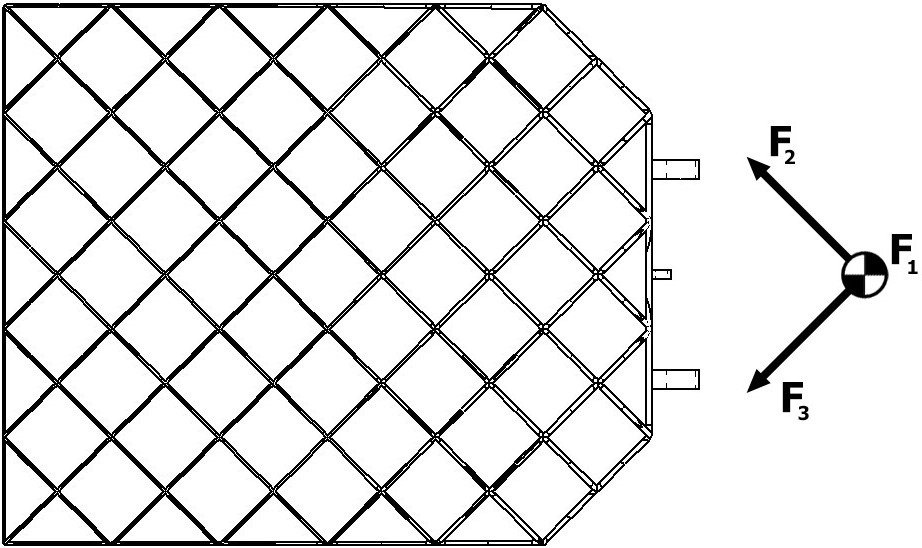
\includegraphics[width=0.6\textwidth]{Gitter.jpg}
	\caption{Kräfte im Grid Fin festen Koordinatensystem}
	\label{abb_gitter}
\end{figure}\\
Somit ergeben sich die Kräfte für die einzelnen Grid Fins zu:
\begin{table}[ht]
	\centering
	\begin{tabular}{c||c|c|c|c}
		&D1&R1&D2&R2\\
		\hline
		$F_1/$N&$413,5$&$389,3$&$389,3$&$413,5$\\
		$F_2/$N&$6276,0$&$4970,8$&$-4970,8$&$-6276,0$\\
		$F_3/$N&$4934,0$&$6474,2$&$-6474,2$&$-4934,0$\\
	\end{tabular}
\end{table}\\~\\
Als Randbedingung werden die Innenflächen der Halterung zylindrisch festgelegt. Das heißt die dort liegenden Knoten können sich weder axial noch radial bewegen, jedoch um die Achse drehen.
\subsection{Optimierung der Halterung}
Bei beiden Pfeilungstypen lässt sich für alle Lastfälle sofort erkennen, dass es zu massiven Lastspitzen an der Halterung kommt. Währenddessen bleiben die Werte im Gitter deutlich niedriger. Der Grund für die hohen Spannungen an der Einspannung ist die nachteilige Lage in der Mitte der Wände anstatt der Schnittstellen, Somit bilden sich vergleichsweise hohe Biegemomente in den Wänden aus. Dieser ungünstige Kraftfluss wird durch die scharfen Kanten weiter verschlimmert. Um nun diese Spannungsspitzen zu vermeiden, sollte, neben einer Abrundung der Kanten, die Position der Halterungen verändert werden.
\begin{figure}[h] 
	\centering
	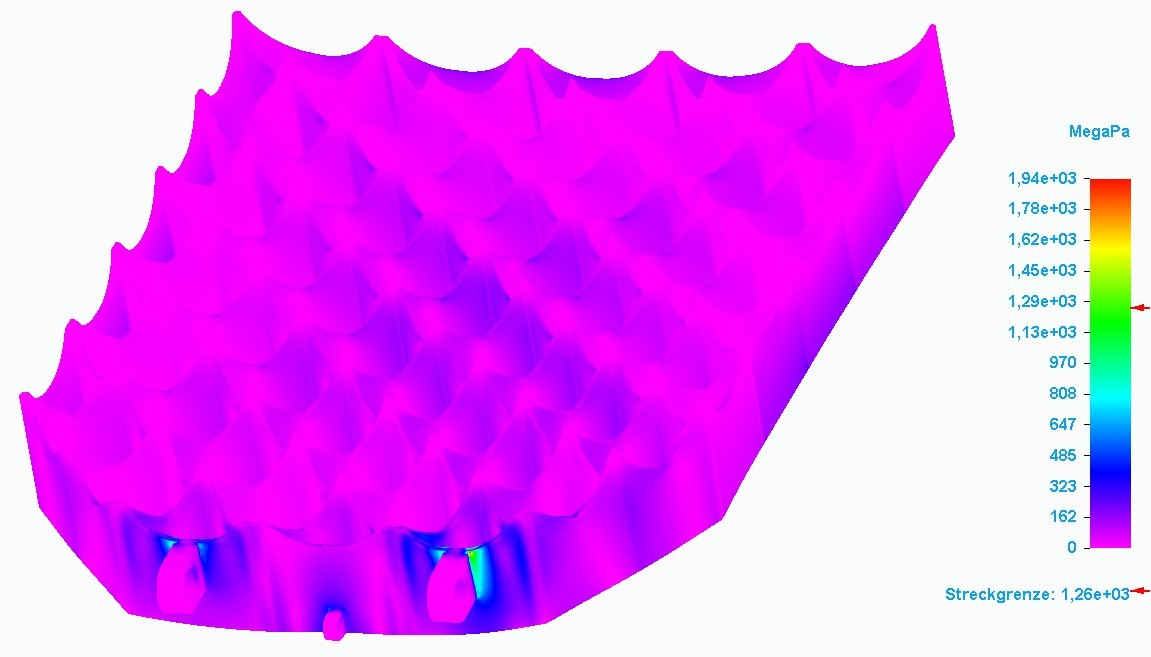
\includegraphics[width=0.9\textwidth]{D1 3.3b max 1.jpg}
	\caption{Maximale Spannungen am Grid Fin D1}
\end{figure}\\
Da sich die Anbringung der Halterungen genau in der Mitte einer gedachten Zelle befinden, die jedoch vom Rahmen halbiert wurde, lassen sie sich entweder tangential oder normal zum Raketenkörper verschieben, um sie auf einen Schnittpunkt der Wände zu legen. Soll Halterung B nicht in zwei Teile aufgeteilt werden, so kommt für sie nur eine Bewegung senkrecht zum Körper in Frage. Anstatt die Halterung nun in das Gitter hinein zu legen, was zu einer Verkleinerung der durchströmten Querschnittfläche führen würde und somit geringer Normalkräfte bewirkt, werden zwei der Wände weiter fortgesetzt. Diese schneiden sich dann in der Mitte, wo die Halterung B platziert wird. Diese Halterung wird jedoch nicht direkt an der Schnittstelle konstruiert, sondern noch ein bisschen weiter vom Gitter entfernt, sodass die Kraft gradliniger über die Beiden Hubstangen geleitet werden kann.

Für die Halterungen A passiert das gleiche. Die nebenliegenden Gitterwände werden bis zu ihrer Schnittstelle fortgesetzt. Im Gegensatz zur Halterung B befindet sich jedoch direkt hier die Bohrung, an der der Grid Fin montiert werden soll.
\begin{figure}[h]
	\begin{minipage}[t]{0.45\linewidth}
		\centering
		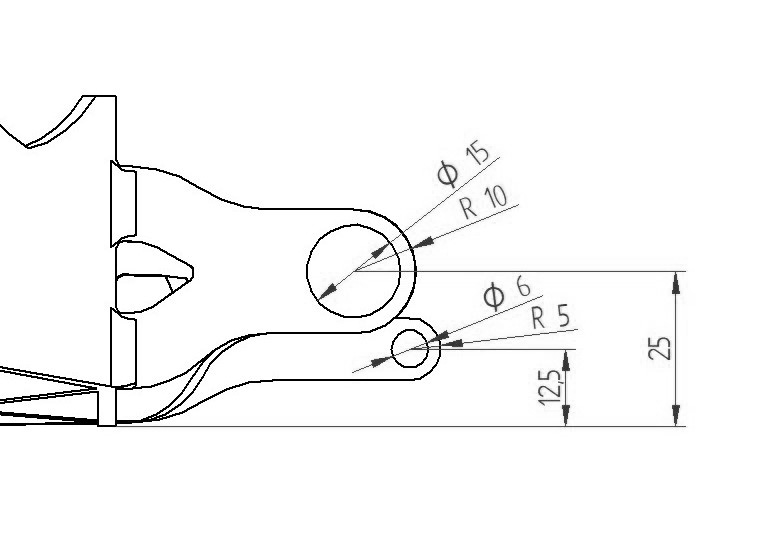
\includegraphics[width=0.85\textwidth]{Skizze Halterung 2.0 1.jpg}
	\end{minipage}
	\hfill
	\begin{minipage}[t]{0.45\linewidth}
		\centering
		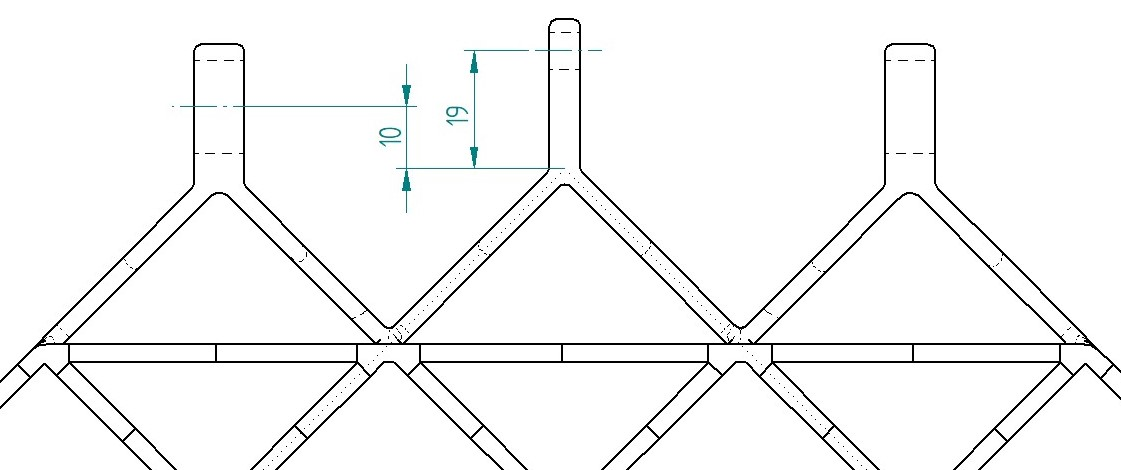
\includegraphics[width=1\textwidth]{Skizze Halterung 2.0 2.jpg}
	\end{minipage}
	\caption{Abrücken der Halterung vom Rahmen}
\end{figure}\\
Dies sorgt zwar schon für eine deutlichere Verbesserung, jedoch ist der Hebelarm trotz der Versetzung der Halterung B recht kurz. Dies sorgt dafür, dass direkt an der Bohrung noch immer Spannungsspitzen auftreten, die die Streckgrenze von $R_{p, 0.2} = 1262$MPa unterschreiten.
\begin{figure}[h] 
	\centering
	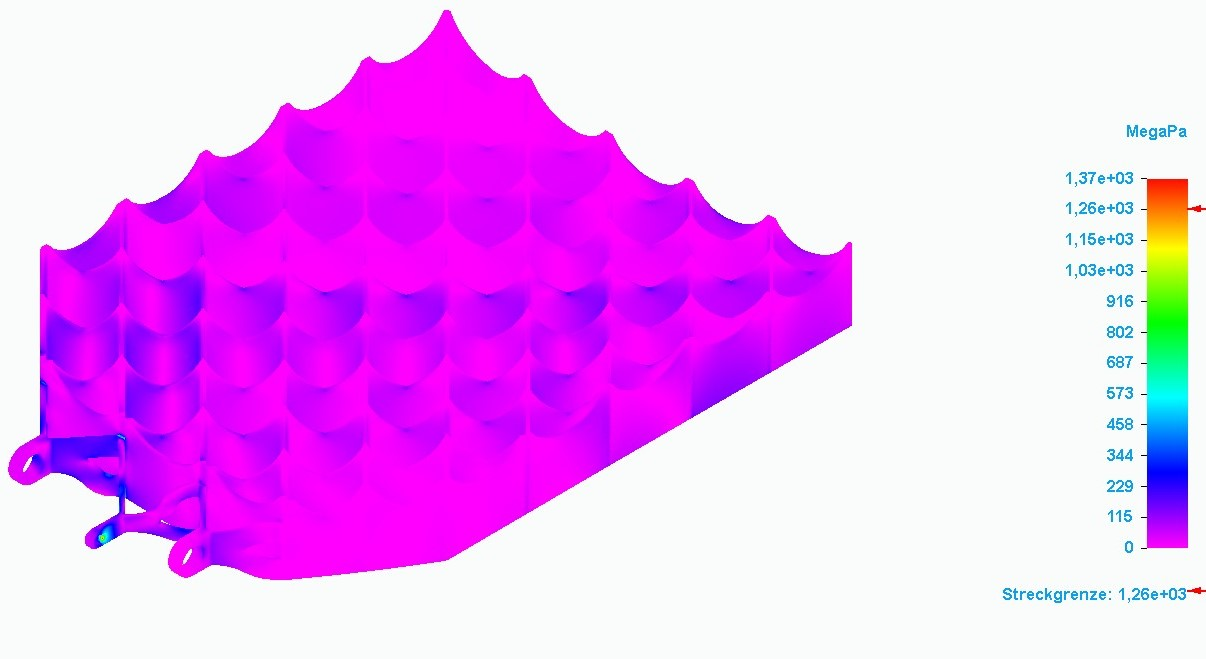
\includegraphics[width=0.9\textwidth]{D2 3.4 b max.jpg}
	\caption{Maximale Spannungen am Grid Fin D2 bei abgerückter Halterung}
\end{figure}\\
Um dem Hebelarm zu verlängern wird nun die Halterung B auf die Höhe der konvexen Seite gebracht. Sie wird außerdem in einer geschwungenen Form noch weiter nach vorne gelegt, damit die Verbindungslinie der beiden Halterungen im $45^\circ$ Winkel zur Gitterebene liegt. Dadurch ist die Klappbewegung möglichst gleichmäßig, was den Aktuator schont und gleichzeitig garantiert, dass der Verfahrweg minimal für den gegeben Hebelarm ist.
\begin{figure}[h] 
	\centering
	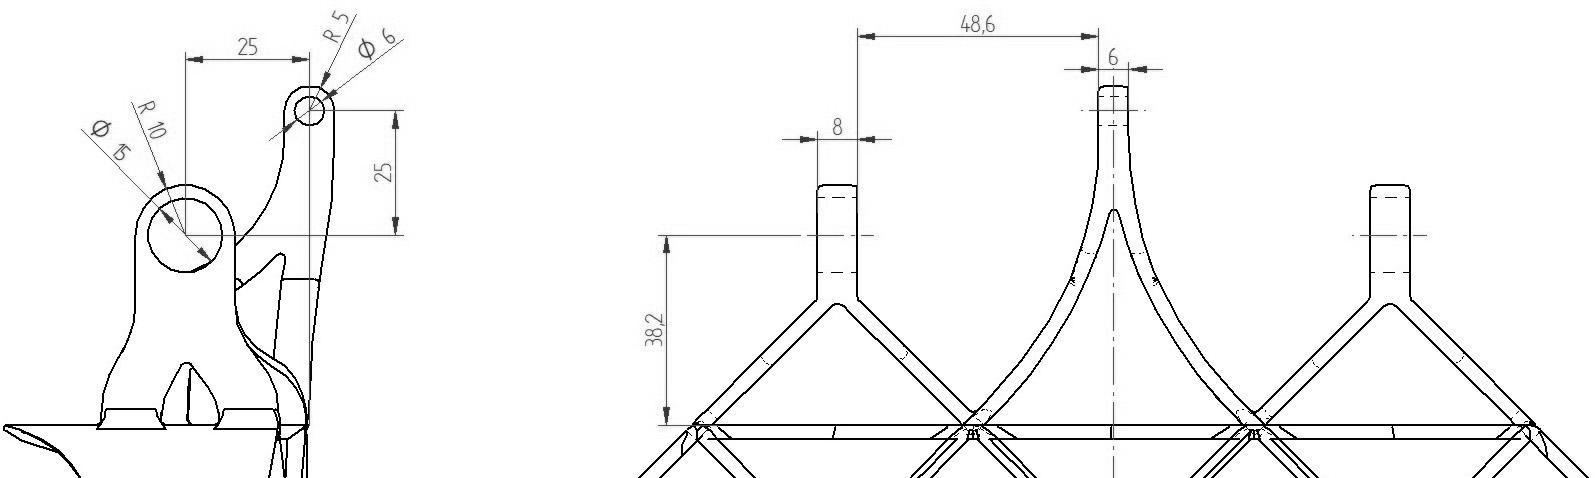
\includegraphics[width=0.9\textwidth]{Skizze Halterung 3.5.jpg}
	\caption{Halterung mit verlängertem Hebelarm}
\end{figure}\\
Dies hat nun endlich den gewünschten Effekt, dass die Spannung im Material deutlich niedriger werden. Bei allen Grid Fins treten nur noch Spannungen auf die deutlich unter der Streckgrenze des Materials liegen und somit den Belastungen im Einsatz standhalten.
\begin{figure}[h] 
	\centering
	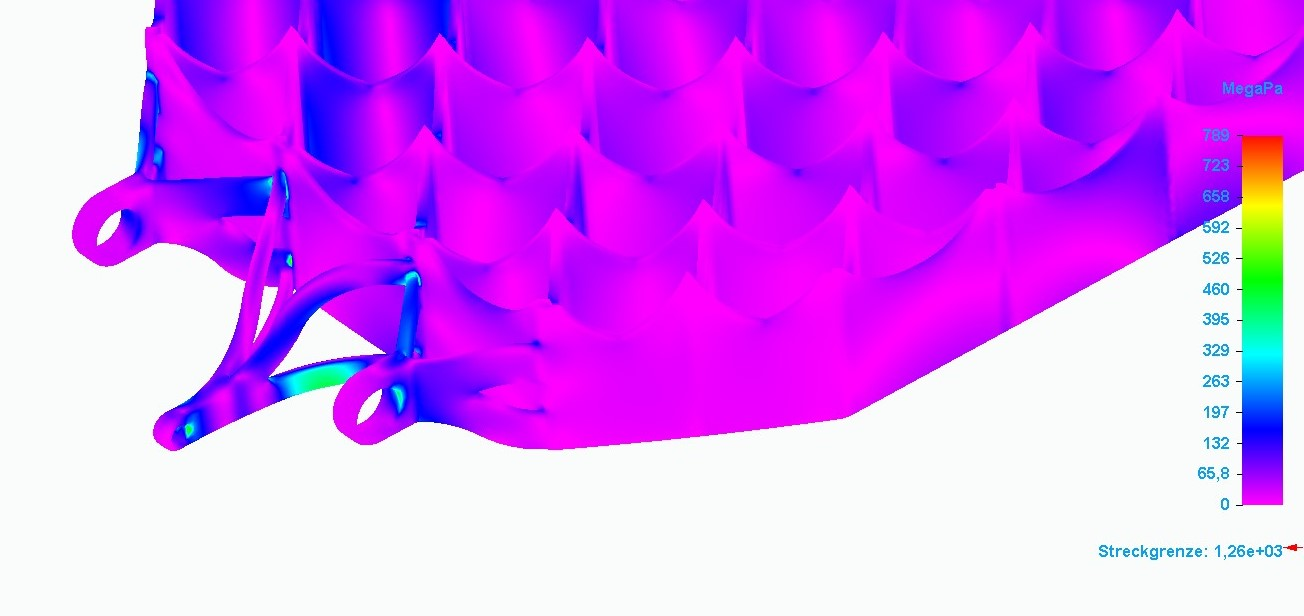
\includegraphics[width=0.9\textwidth]{3.5 b Halterung max.jpg}
	\caption{Maximale Spannungen am Grid Fin D2 bei der Halterung mit verlängertem Hebelarm}
\end{figure}\\
Somit wäre die Auslegung der Halterung nach den aerodynamischen Kräften theoretisch abgeschlossen, jedoch muss hierbei auch noch auf die Aktuatorik und das maximale Lastenvielfache geachtet werden. Aktuell hat der Grid Fin eine Masse von $m = 3,5$kg und der Massenschwerpunkt liegt $185$mm von der Halterung A entfernt. Mit dem Lastenvielfachen von ca. 20 beim auslösen des Ballutes entsteht nun also ein Moment von ungefähr $M=127Nm$, welches von der Halterung B kompensiert werden muss. Die Halterung B ist an der Spindelstange montiert und leitet somit die Kraft an diese weiter. Der Hebelarm der Halterung B und die maximale ertragbare Axialkraft der Spindel müssen also aufeinander abgestimmt sein. Maxon Motoren stellt nur Spindeln mit Axiallasten von bis zu $2700$N her, welche folglich einen Hebelarm von $\frac{127Nm}{2700N}=47mm$ erfordert, was noch gerade so für den Grid Fin annehmbar ist, weshalb ein Exemplar von diesem Anbieter gewählt wird. Der Wert liegt laut dieser Rechnung zwar minimal drüber jedoch wird das Lastenvielfache von 20 gar nicht wirklich erreicht, sodass die Rundung annehmbar ist. Da die Hubstange gelenkig mit dem Grid Fin verbunden ist, ist zu beachten, dass nur der Abstand der Haltungen in Sehnenlänge als effektiver Hebelarm wirkt. Somit muss die Halterung B nicht länger weiter vorne positioniert sein, da für den Grid Fin so weniger Material und Bauraum benötigt wird. Wird die Verbindungsstange zwischen Halterung und Hubstange auf die gleiche Länge wie der Hebelarm gesetzt, verlängert sich auch nicht der Hub und da die Hubstange sich nun im eingeklappten Zustand weiter außerhalb der Rakete befindet, braucht sie auch weniger Platz innerhalb, wenn der Grid Fin ausklappt. Um auf den gewünschten Hebelarm zu kommen werden nun beide Halterungen noch ein wenig nach außen gelegt, sodass sich die endgültige Geometrie, wie sie in Abbildung \ref{abb_Halterung-fertig} zu sehen ist, ergibt. Zusätzlich befinden sich noch Kanten und Nuten zur Befestigung der Lagerung, aber auf diese wird erst später im Detail eingegangen.
\begin{figure}[h] 
	\centering
	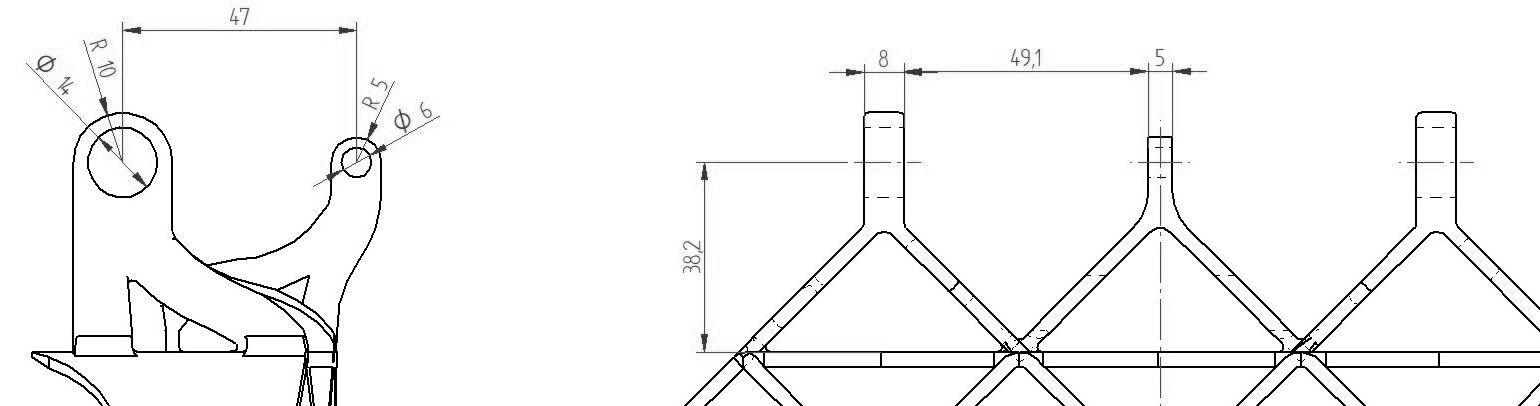
\includegraphics[width=0.9\textwidth]{Skizze Halterung 3.6.jpg}
	\caption{Endgültige Geometrie der Halterung}
	\label{abb_Halterung-fertig}
\end{figure}\\
Zur Bestätigung werden wieder FEM Analysen durchgeführt und diesmal werden ergänzend zu den aerodynamischen Kräften auch in einem separaten Lastfall die Beschleunigungskräfte untersucht. Bei den Lastvielfachen werden die anderen Kräfte ignoriert, da sie eher eine Stützwirkung habe und somit die Spannungen nur weiter senken würde. Beim Auftreten der ruckartigen Abbremsung durch den Ballonschirm ist der Max Q ohnehin schon überschritten und somit sind die anderen Kräfte nur noch deutlich geringer. Wie Abbildungen \ref{abb_Halterung_max} und \ref{abb_Halterung_20g} zeigen wird die Streckgrenze weiterhin nicht unterschritten. Somit gibt die Halterung als bestätigt.
\begin{figure}[h]
	\begin{minipage}[t]{0.5\linewidth}
		\centering
		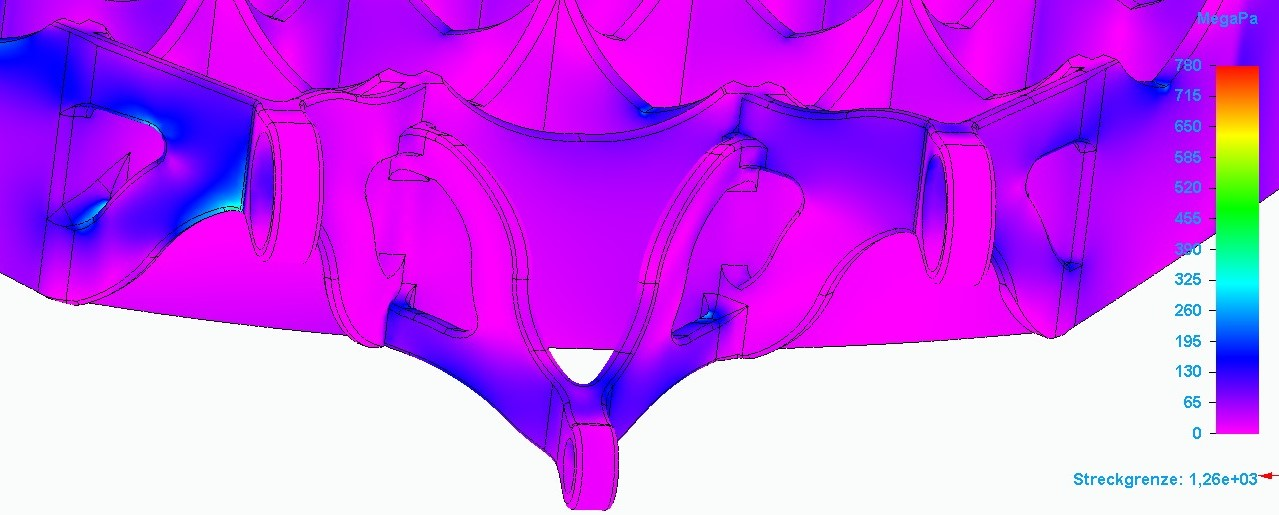
\includegraphics[width=0.95\textwidth]{D2 3.6.2 b Halterung.jpg}
		\caption{Maximale Belastungen an der entgültigen Geometrie der Halterung}
		\label{abb_Halterung_max}
	\end{minipage}
	\hfill
	\begin{minipage}[t]{0.41\linewidth}
		\centering
		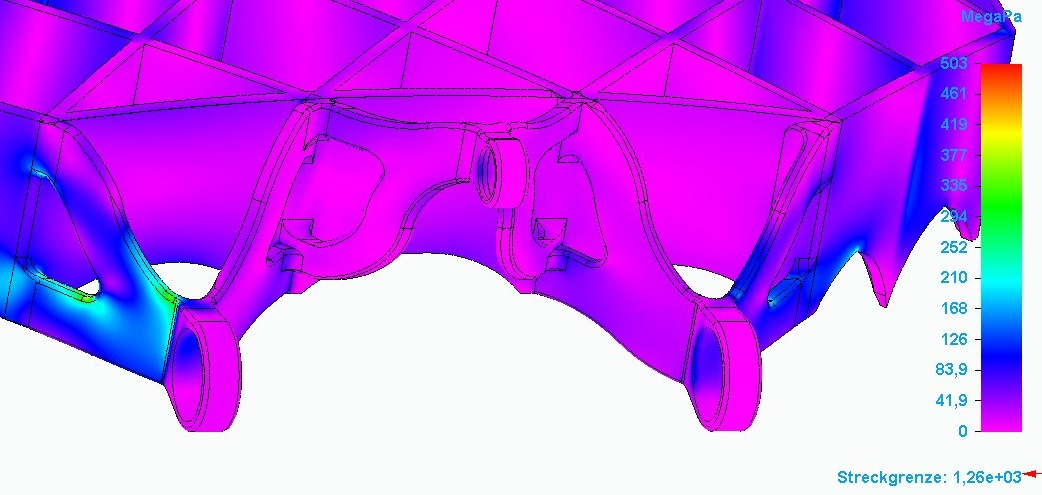
\includegraphics[width=\textwidth]{20g 3.6.2 b.jpg}
		\caption{Belastungen an der entgültigen Geometrie der Halterung beim Lastenvielfachen}
		\label{abb_Halterung_20g}
	\end{minipage}
\end{figure}
\subsection{Optimierung des Gitters}
Als nächstes wird das Gitter untersucht. Es ist sofort erkenntlich, dass die Belastungen überall relativ niedrig und deutlich unter der Streckgrenze liegen. Egal ob beim Tal- oder Berg-Typus, die Spannungsspitzen, die auftreten, sind keines Wegs kritisch. Somit ist eine Aufdickung des Material nicht nötig, sondern es kann über eine Reduzierung der Wandstärke nachgedacht werden.

Die Wanddicke ist aber nicht nur durch die mechanischen Belastungen, sondern auch die thermischen, nach unten hin beschränkt. Diese ist jedoch ein sehr komplexes Phänomen, das von der Zusammensetzung der Atmosphäre, den zeitlich ändernden Strömungsbedingungen, der Position des Verdichtungsstoßes und dem Aufbau des Grid Fins abhängt, sodass es nicht auch nur überschlägig in dieser Arbeit behandelt wird.
\\~\\
Der Grid Fin ist momentan am von der Rakete weg zeigenden Ende nur $1,5$mm dick, was für den Wiedereintritt schon ein relativ kleiner Wert sein könnte. Deswegen soll dieser zunächst nicht unterschritten werden. Es ist jedoch auch kein signifikanter Anstieg der Spannungen zu zur Halterung hin zu erkennen, der den Verlauf der Wanddicke rechtfertigt. Deswegen werden zunächst alle Wände im Gitter auf eine Dicke von $d_G = 1,5$mm gesetzt, während die Wandstärke und die Wände, die außerhalb des Gitters zu den Halterungen führen unverändert bleiben. Dies scheint nach einer ersten FEM-Analyse die Belastung des Materials nicht stark zu verändern, sodass auch Rahmen- und Halterungswände auf diesen Wert hinab gesetzt werden. Die Spannungen in den Grid Fins liegen für alle Positionen und auch beim maximalen Lastenvielfachen weit unter der Streckgrenze von $R_{p, 0.2} = 1262$MPa. Die höchsten Spannungen treten beim Grid Fin des Tal-Typus in der Position D2 auf. 
\begin{figure}[h] 
	\centering
	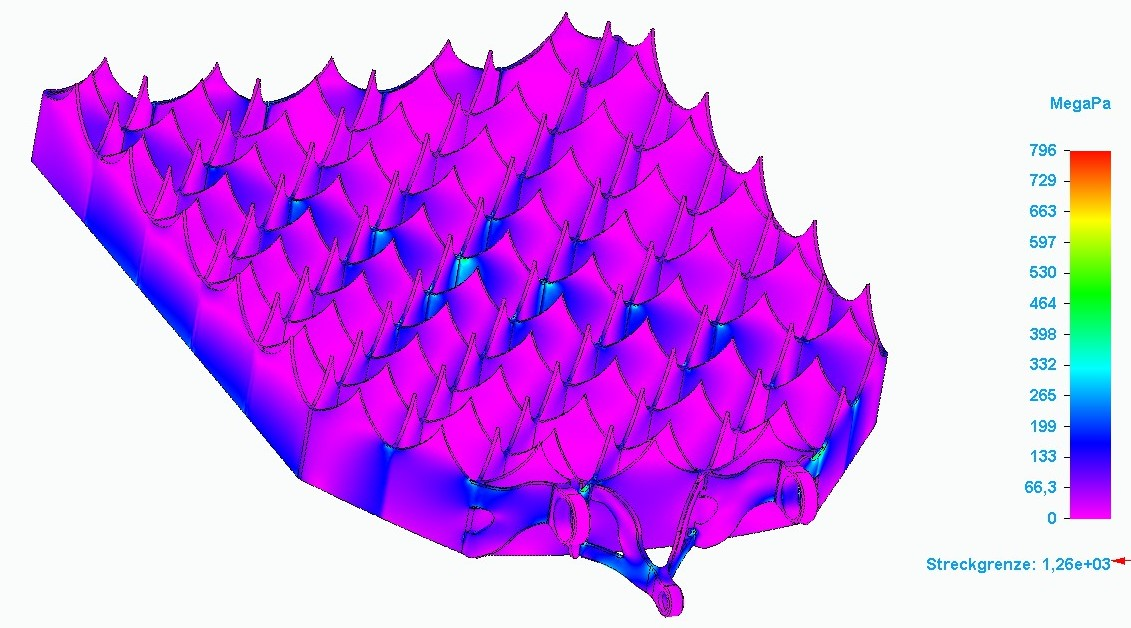
\includegraphics[width=0.8\textwidth]{D2 3.9 t.jpg}
	\caption{Maximale Spannungen für konstante Wanddicke von $1,5$mm}
\end{figure}\\
Somit resultiert ein Sicherheitsfaktor von über 1,5. So hohe Spannungen treten jedoch nur an einzelnen Stellen auf, die hauptsächlich am Berührungspunkt der Halterung mit dem Rahmen oder direkt an der Halterung liegen. Im Gitter sind für alle Belastungsfälle die Spannungen geringer und bleiben großteils unter 200MPa. Deutlich sind außerdem zwei diagonale Streifen, die sich in der Mitte des Gitters treffen, zu erkennen, in denen ebenso wie am Rahmen etwas höhere Belastungen auftreten. Aber selbst das Maximum in der Mitte ist mit Spannungen knapp über 300MPa noch immer ungefährlich.
\\~\\
Der Vergleich von der Berg- und Tal-Konfiguration zeigt, das keine signifikanten Unterschiede auftreten. Die maximalen Spannungen sind beim Tal-Typus zwar immer etwas größer, aber nur um so kleine Beträge, dass es keine Rolle spielt. Deswegen muss an der Stelle wieder thermisch argumentiert werden. Beim Tal-Typus sind die Spitzen isolierte der Strömung entgegenzeigende Punkte. Beim Berg-Typus hingegen, liegen die Spitzen der sich kreuzenden Wände aufeinander, sodass die Wärme an ein größeres Volumen abgegeben werden kann. Unter der Annahme, dass der Berg-Typus somit thermische robuster ist, wird dieser hier als die endgültige Geometrie des Grid Fins ausgewählt. Seine finale Masse beläuft sich somit auf $2,8$kg, was somit auch dafür sorgt, dass die Spindelstange einen ausreichenden Sicherheitsfaktor hat.
\\~\\
Eine ergänzende vollständige Sammlung der Ergebnisse der FEM-Analysen aller Belastungszustände am Grid Fin befindet sich im Anhang \ref{sec:mehrFEM}.
An dieser Stelle sein noch zusätzlich zu erwähnen, dass folglich auch die Ideen zur Integrierung von Hohlräumen verworfen werden müssen. Egal ob zur Kühlung, Druckmessung oder einfach nur Gewichtseinsparung, die geringe Wanddicke erlaubt keinen Platz für solche Strukturen.
\section{Bestätigung mechanischen Belastbarkeit der Aktuatorik}
Nun der Aufbau des Grid Fins, insbesondere der Halterung feststeht, kann überprüft werden, ob auch alles auf der Wellenseite den mechanischen Lasten standhält. Hierfür werden die Kräfte, die an den einzelnen Halterungen wirken benötigt. Die detaillierte Rechnung befindet sich im Anhang \ref{sec:halterkraefte}. Wenn angenommen wird, dass die Halterung B, da sie deutlich weniger steif als die Halterungen A sind, nur Belastung in $\eta$-Richtung aufnehmen kann ergeben sich die Kräfte wie folgt. Links sind Kräfte am Grid Fin R1 dargestellt, was die höchste Belastung für das Lager A bedeutet, und rechts R2 mit der höchsten Belastung für Lager B.
\begin{figure}[h] 
	\centering
	\includegraphics[width=0.5\textwidth]{Halterungkräfte1.png}
	\caption{Kräfte an den Halterungen}
\end{figure}
\begin{table}[h] 
	\centering 
	\begin{tabular}{c|c|c|cc||c|c|c|c} 
		\textbf{R1}&$F_{\zeta}$[N]&$F_\eta$[N]&$F_\xi$[N]&&\textbf{R2}&$F_{\zeta}$[N]&$F_\eta$[N]&$F_\xi$[N]\\ 
		\hline 
		A1& 612,00&-5601,54&-531,55&&A1&599,90&5,16&-474,45\\
		A2&-1001,31&-1624,49&-531,54&&A2&.1013,41&3554,87&-474,45\\
		B&0&-886,81&0&&B&0&4366,53&0\\
	\end{tabular}
\end{table} \\
Für die Bauteile, die nicht so hohen Lasten wie der Grid Fin ausgesetzt sind, wird im Folgenden nicht mit den Werkstoffwerten des teuren Edelstahls 1.4542 gerechnet. Für die Teile, die nicht mit der Strömung in Kontakt kommen, wird stattdessen eine Aluminiumlegierung mit $R_{p,0.2} = 280$MPa verwendet, und für die anderen Bauteile, wie weiterhin auch hohen thermischen Lasten ausgesetzt sind, wird ein Edelstahl mit einer Streckgrenze von $R_{p,0.2} = 400$MPa angenommen.
\subsection{Lager der Halterung}
Für die Lasten an den Lagern ist nur die Aufteilung in Radial- $F_r$ und Axialkraft $F_a$ von Bedeutung. Dabei sei noch zu bedenken, dass die Kraft in $\xi$-Richtung auf Grund des Aufbaus nur von einem der A Lager kompensiert werden kann. Auch wenn das für die vorherige Berechnung keine Rolle spielte, da die beiden Halterungen A auf einer Achse liegen, wird es im Folgenden berücksichtigt.
\begin{table}[h] 
	\centering 
	\begin{tabular}{c|c|cc||c|c|c} 
		\textbf{R1}&$F_{r}$[N]&$F_a$[N]&&\textbf{R2}&$F_{a}$[N]&$F_r$[N]\\ 
		\hline 
		A1& 5634,87&-1063,10&&A1&599,92&948,90\\
		A2&1908,29&0&&A2&3696,60&0\\
		B&866,81&0&&B&4366,53&0\\
	\end{tabular}
\end{table} \\
Aus diesen Werten lässt sich nun über die Flächenpressung und Abscherung den erforderlichen Durchmesser $D$ und die benötigte Auflagebreite $B$ der Hilfswelle bestimmen. Für die Abscherung git
\begin{equation}
	\tau_{\mathrm{zul.}}\leq\tau_\mathrm{scher}=\frac{F_r}{m\pi D^2/4}.
\end{equation}
Mit $\tau_{\mathrm{zul.}}=R_{p, 0.2}\cdot 0,6$ \cite{metall} und $m$ als die Anzahl der Schnittflächen lässt sich der Mindestdurchmesser bestimmen.
\begin{equation}
	D \leq \sqrt{\frac{4F}{m\pi 0,6 R_{p, 0.2}}}= 5,5\mathrm{mm}
\end{equation}
Für die Halterung A ist $m=1$, sodass eine Mindestdicke von $D=5,5$mm benötigt wird. Aus der sich eine Auflagebreite von $B = 3,1$mm ergibt. Da sich der Aufbau des Grid Fins seit dem ersten Modell verändert hat, muss auch die Anbringung an der Welle, welche in Abbildung \ref{abb_Welle} zu sehen war, angepasst werden. Durch wie Verlegung der Halterung A rückt der Grid Fin näher an den Raketenkörper ran. Statt nun Greifarme aus der Welle raus ragen zu lassen, wir diese nur ein wenig verlängert, sodass die Verbindungslinie durch die beiden Halterungen A die Welle durchstößt. Auf diese Verbindungslinie wird eine Stange mit einem Durchmesser von $D = 10$mm, im weiteren Verbindungswelle genannt, gelegt, auf der der Grid Fin montiert wird. Diese Variante der Halterung hat zum einen den Vorteil, dass keine komplizierte Greiferstruktur gefertigt werden muss, und zum anderen steht nun ein Großteil der planaren Rahmenwand im eingeklappten Zustand nicht mehr direkt in der Strömung, sondern im Windschatten der Welle. Dadurch wird ungewollter Widerstand und Belastung der Grid Fins verhindert. Um den Grid Fin reibungsarm zu sicher, muss er sowohl axial als auch radial mit Wälzlagern gelagert werden. Zylinderrollenlager, wie sie schon bei der Welle verwendet werden, sind hier jedoch eine ungünstige Wahl, da sie einen recht großen Bauraum benötigen. Stattdessen wird die Halterung A auf beiden Seiten mit einem schmalen Nadellager radial und mit einem Kugellager axial mit der Welle verbunden. Diese Kombinationslager werden von außen mit Nutmuttern, die auf die Verbindungswelle aufgeschraubt und durch Sicherungsbleche gesichert werden, an den Grid Fin gedrückt. Um ein Verrutschen der Verbindungswelle in der Welle zu verhindern, muss diese noch durch eine Passschraube fixiert werden. Für diese Passschraube werden wieder aus der Flächenpressung und der Abscherung die Mindestmaße des Durchmessers und der Breite bestimmt. Mit einem Durchmesser von $D = 10\mathrm{mm}> 1,2$mm und einer Kontaktbreite von $B = 8\mathrm{mm}> 1,3$mm ist sie für diese Anwendung ausreichend.
\begin{figure}[h] 
	\centering
	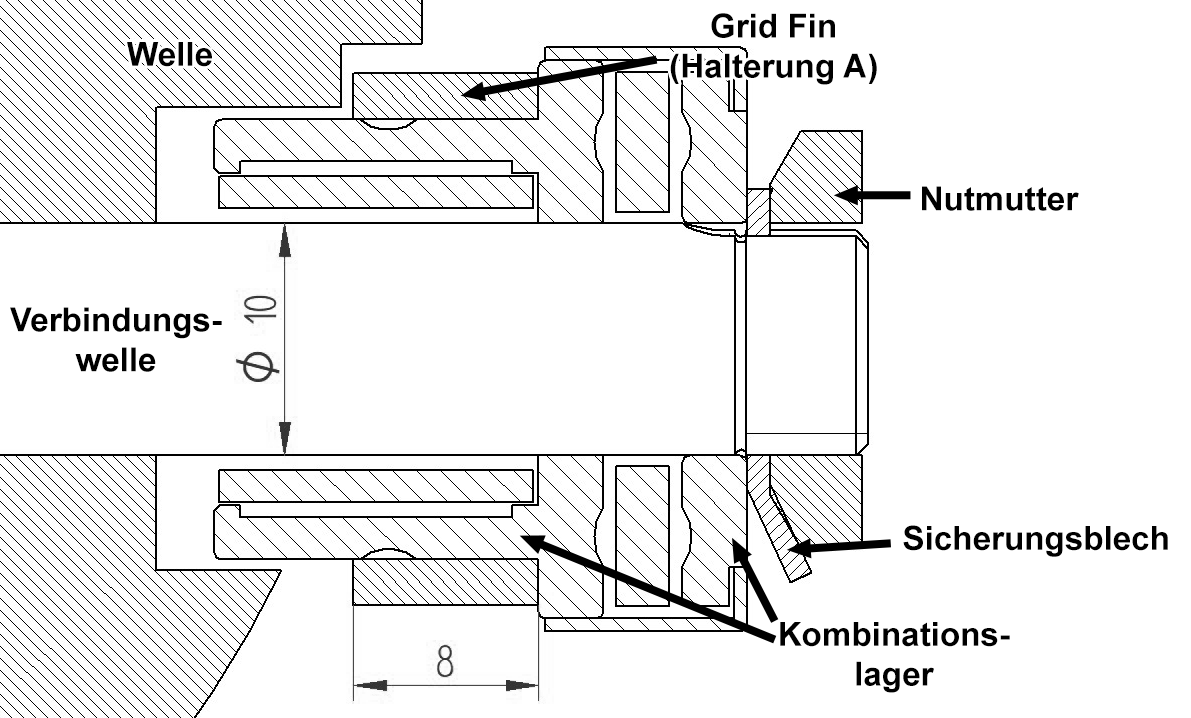
\includegraphics[width=0.75\textwidth]{Skizze Halterung A.png}
	\caption{Lagerung der Halterung A}
\end{figure}\\
Die Halterung B wird von beiden Seiten gestützt, sodass mit $m = 2$ ein Mindestdurchmesser von $D = 3,4$mm errechnet wird. Die zugehörige Breite beläuft sich somit auf $B = 3,8$mm. Wie schon angemerkt treten hier kaum Axialkräfte auf, sodass ein Rillenkugellager ausreicht, um diese aufzunehmen. Es wird auf der einen Seite gegen eine Schulter in der Halterung B des Grid Fins gedrückt und auf der anderen Seite durch ein Sicherungsring fixiert. Zwei Stifte werden von beiden Seiten gegen die innere Kante des Lagers gedrückt und miteinander verschraubt. Diese Stifte können anschließend von außen mit Muttern an die Verbindungsstange für den Hub fixiert werden. Somit ist auch die Halterung B axial und radial bestimmt, kann sich aber noch immer reibungsarm um ihre Achse drehen. Das Kugellager hat zwar nur eine Breite von 3mm, was unter dem Wert liegt, der sich aus der Flächenpressung ergeben hat. Jedoch wurde dort mit dem Mindestdurchmesser gerechnet, sodass, wenn mit dem Innendurchmesser des Kugellagers von $D = 5$mm die Rechnung wiederholt wird, nur noch eine Breite von $B =2,6$ benötigt wird. Diese Lagerung wird genauso auch ein zweites Mal auf der anderen Seite der Verbindungsstange verwendet.
\begin{figure}[h] 
	\centering
	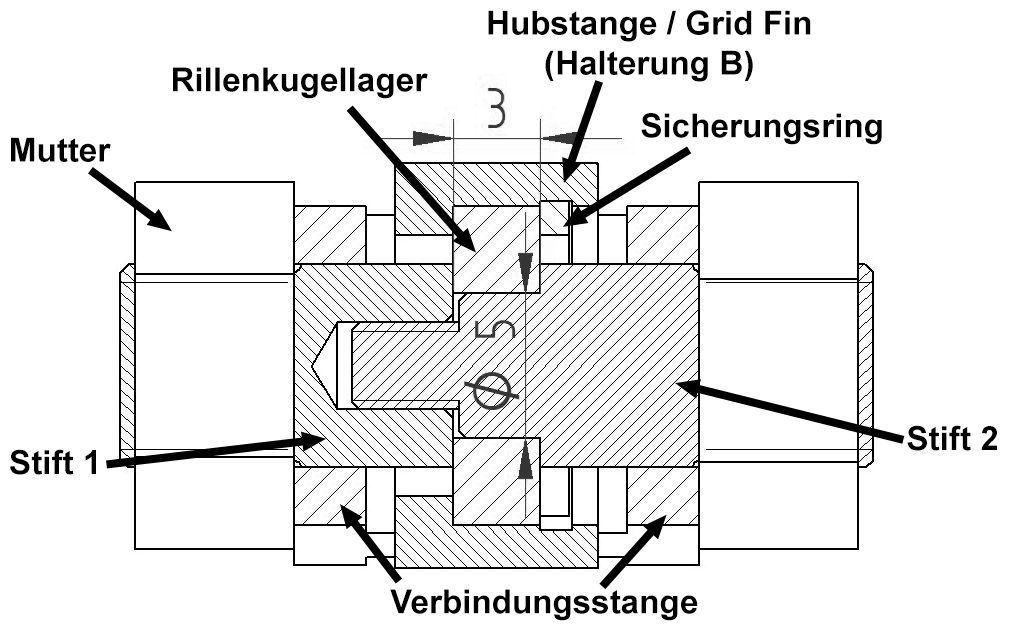
\includegraphics[width=0.75\textwidth]{Skizze Halterung B.png}
	\caption{Lagerung in der Halterung B}
\end{figure}
\subsection{Lagerung der Welle}\label{sec:lagerWelle}
Als nächstes wird die Lebensdauer der Lagerung der Welle überprüft, da diese sich auch unter Last bewegen müssen. Hierzu werden zunächst über das Kräftegleichgewicht die Lasten in den beiden Kegelrollenlagern bestimmt.
\begin{figure}[h] 
	\centering
	\includegraphics[width=0.9\textwidth]{Skizze Lager.png}
	\caption{Lagerkräfte an den Kegelrollenlagern}
\end{figure}\\
Für den Fall, dass die am Grid Fin angreifende Axialkraft in positive $\eta$-Richtung zeigt, ist die Axialkraft am vorderen Kegellager $F_{a, \mathrm{K1}} = 0$ und am hinteren $F_{a, \mathrm{K2}} = F_\eta$. Da es für den anderen Fall genau umgekehrt ist, wird bei der Untersuchung der maximalen Belastung für beide Lager angenommen, dass sie jeweils die Axiallast aufnehmen. Die Radialkräfte ergibt sich aus der Kraft in $\zeta$- und $\xi$-Richtung und lässt sich mit dem Kräfte- und Momentengleichgewicht bestimmen.
\begin{equation}\label{eq_lagerWelle1}
	F_{r, \mathrm{K1}} = F_r\cdot\frac{208\mathrm{mm}}{265\mathrm{mm}}=6359,5\mathrm{N}
\end{equation}
\begin{equation}\label{eq_lagerWelle2}
	F_{r, \mathrm{K2}} = F_r-F_{r, \mathrm{K1}}=1742,7\mathrm{N}
\end{equation}
Aus den Lasten in den Lagern und den in den Herstellerangaben genannten statischen Tragzahlen lässt sich die äquivalente Belastung berechnen. Mittels der ebenfalls vom Hersteller gegebenen dynamische Tragzahl ergibt sich dann für beide Lager eine Lebensdauer vom mehreren tausend Stunden \cite{metall}. Es wurde dabei mit der maximal auftretenden Drehzahl, die sich aus der in Kapitel \ref{sec:betriebssim} beschriebenen Betriebssimulation ergibt, gerechnet. Trotzdem liegt der Wert noch immer deutlich über der benötigten Lebensdauer. Dies liegt jedoch daran, dass die Größe der Lager sich aus der Geometrie der Welle und des Grid Fins anstatt aus den Belastungen ergeben hat, wodurch kein kleines Modell in Frage kommt. Bei den gewählten Exemplaren wurde schon versucht die preislich günstigste Option zu wählen, sodass sie ihre Größe nicht zu sehr zum Nachteil wird.
\subsection{Belastung der Welle}
Die Welle selbst hat zum einen den groben Verlauf, wie er in Abbildung \ref{abb_Welle} zu sehen war, zum anderen weicht sie an einigen Stellen von dieser rotationssymmetrischen Geometrie ab. Ein Aspekt ist die schon im Abschnitt zu der Halterung angesprochenen Verbindungswelle, die die Welle durchstößt. Auf der gleichen Höhe, aber auf der Stirnseite befindet sich mittig eine Bohrung und Senkung für die Passfeder. Für die Hubstange existiert des Weiteren ein großer Ausschnitt durch den größten Durchmesser der Welle. Damit im eingeklappten Zustand die Berge des Grid Fins nicht gegen die Welle stoßen, ist die untere Vorderkante ausgehöhlt. Das Linearlager der Hubstange muss von unten festgeschraubt werden, sodass zunächst ein flacher Ausschnitt in die Welle eingebracht ist, auf der eine Platte festgeschraubt werden kann. Diese Platte wird anschließend von unten mit dem Lager verschraubt. Um ein montieren der Schrauben zu ermöglichen werden jedoch noch Einbuchtungen an der Welle benötigt. Von den sechs Bohrungen auf der Welle für die Platte sind die hinteren zwei größer Dimensioniert, da dort noch ein weiteres Bauteil montiert werden soll, an dem anschließend die das Spindelgetriebe festschraubt wird.
Für das Spindelgetriebe mit dem integrierten Motor sind auch noch kleine Einbuchtungen in der Welle nötig. Am hinteren Ende befindet sich dann schließlich das Gewinde für die Nutmutter und die Nut für das Sicherungsblech. Schlussendlich befindet sich an der hinteren Stirnseite der Welle eine Bohrung mit Passfedernut in der die Welle des Getriebes montiert wird.
\begin{figure}[h] 
	\centering
	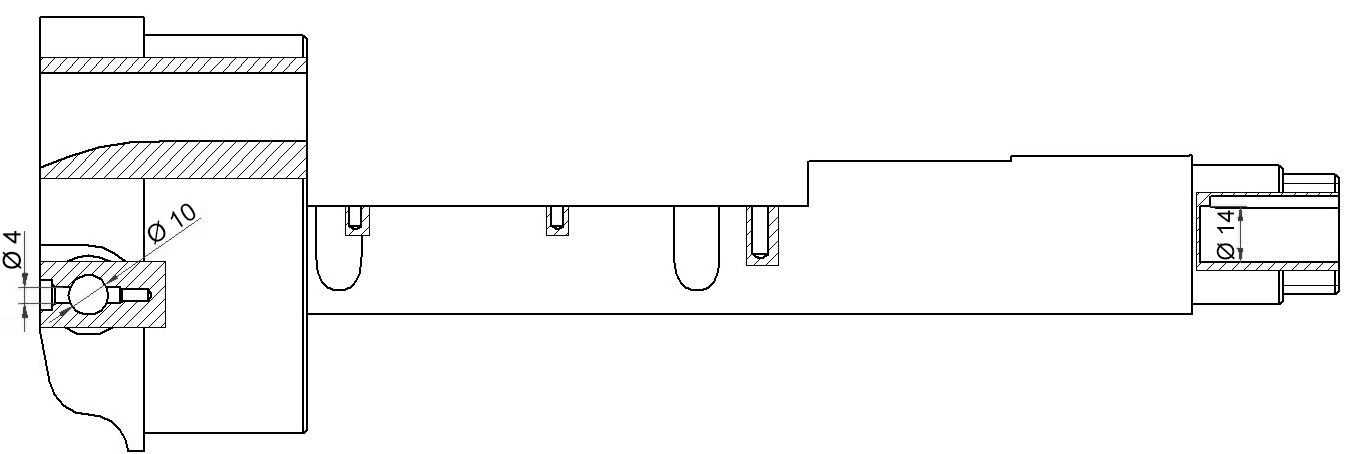
\includegraphics[width=0.9\textwidth]{Skizze Welle ausbruch.jpg}
	\caption{Aufbau der Welle}
\end{figure}\\
Für die Analyse der Welle wurden wieder FEM-Berechnungen durchgeführt. Auf den Flächen, wo die Lager aufliegen, wird wie schon beim Grid Fin zylindrische Bedingungen festgelegt, wobei die axiale Beschränkung nur bei jeweils einem der beiden Lager angewandt wird. Zusätzlich wird eine Drehung der Welle um ihre Achse durch ein festhalten in tangentiale Richtung der Passfedernut am hinteren Ende verhindert.
Die Kräfte der Halterung A werden an den Stellen eingeleitet, wo die Verbindungswelle in die Welle führt, mit Ausnahme der $\xi$-Kraft, die durch die Passschraube übertragen wird. 
Die Kraft der Halterung B hingegen wird erst über das Spindelgetriebe auf die Welle übertragen. Somit greift die resultierende Kraft in der Simulation in den Bohrlöchern an, an denen die Spindel befestigt ist.
\begin{figure}[h] 
	\centering
	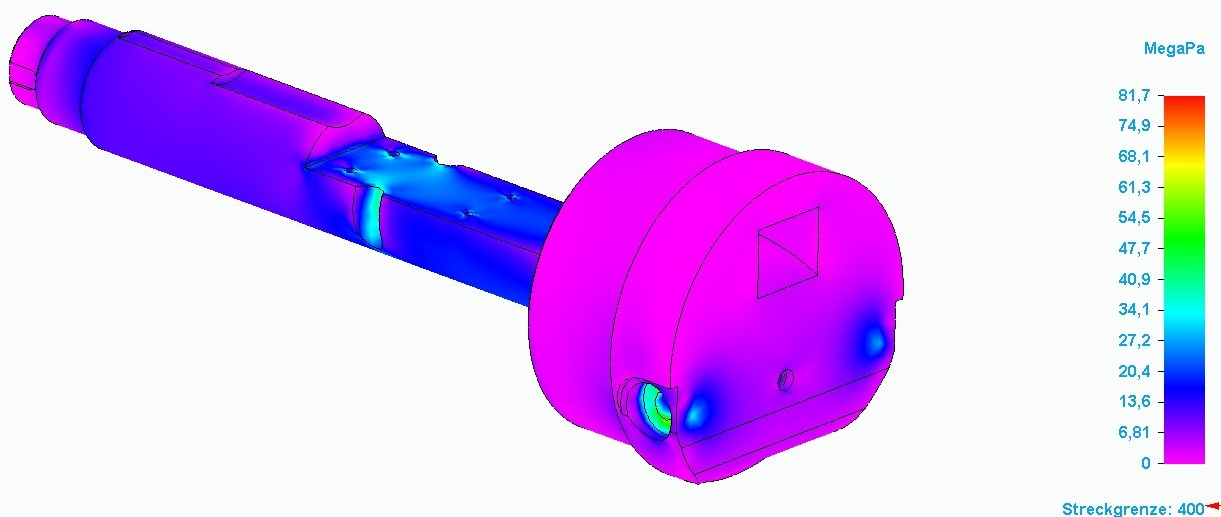
\includegraphics[width=0.9\textwidth]{FEM Welle.jpg}
	\caption{FEM-Ergebnisse der Welle}
	\label{abb_Well_FEM}
\end{figure}\\
Wie auch bei den Lagern, ist die Dimensionierung der Welle nicht durch die mechanischen Lasten sondern geometrischen Randbedingungen bestimmt, sodass nirgends auch nur ansatzweise kritische Belastungen auftreten.

\subsection{Belastung des Gehäuse}
Schlussendlich wird noch das Gehäuse betrachtet. Es hat nicht nur die Aufgabe den Rest der Rakete von den beweglichen Teilen zu trennen, um zum Beispiel ein Verfangen von Kabeln zu verhindern, sondern auch die Funktion die Lager und den Motor mit Getriebe in Position zu halten. Somit überträgt das Gehäuse auch die Kräfte und Momente die in dem System wirken auf den Raketenkörper. Für eine einfache Montage und Fertigung besteht das Gehäuse aus einer Unter- und Oberseite, die mit Schrauben aneinander und an der Außenhülle befestigt werden. Im vorderen Bereich benötigt die Oberseite der Welle auf Grund der Klappaktuatorik deutlich mehr Platz als auf der Unterseite. Deshalb bildet die Oberseite des Gehäuses einen Halbkreis, während die Unterseite eine halbe Ellipse darstellt, deren große Halbachse dem Radius der Oberseite entspricht, um bündig mit ihr abzuschließen. Hinter dem Kegelrollenlager sind beide Seiten symmetrisch aufbaut mit Ausnahme der Trennwände, die zur Unterseite gehören und an denen das Getriebe und der Motor montiert werden. Somit muss bei der Montage als letzter Schritt nur noch die Gehäuseoberseite auf die Unterseite platziert und dann befestigt werden.
Diese Befestigung findet mit der Raketenhülle mit sechs gleichmäßig über einen Flansch verteilte Schrauben statt. Auch miteinander werden die beiden Hälften zunächst auch mit sechs Schrauben, die über die gesamte Kontaktfläche verteilt sind, platziert und mit Mutter befestigt werden.
\\~\\
Auch hier wird wieder eine FEM-Analyse benutzt, um die Spannungen im Material zu bestimmen. Hierbei werden die Lagerkräfte auf die Flächen aufgebracht, auf denen die Lager aufliegen und gegen drücken. Das Moment um die Wellenachse wird über das Getriebe und den Motor auf das Gehäuse übertragen. Da das Getriebe eine Übersetzung von 200:1 besitzt und der Motor nur sehr kleine Momente liefert, wird vereinfacht angenommen, dass das gesamte Moment an Löchern für die Schraube des Getriebes angreift.
\begin{figure}[h] 
	\centering
	\includegraphics[width=0.75\textwidth]{Gehäuse.jpg}
	\caption{Ergebnisse der FEM-Berechnung der Gehäusebaugruppe mit 6 Schrauben}
\end{figure}\\
Die FEM-Analyse zeigt, dass die Beanspruchungen im Material überall recht gering sind. Nur die Schrauben und Mutter werden stark mit Spannungen von bis zu $900$MPa belastet. Dies können Schrauben der Festigkeit 9.8 beziehungsweise 10.9 mit ihrer Zugfestigkeit bzw. Streckgrenze zwar erreichen. Aber da sie als Normbauteile kostentechnisch kaum eine Rolle spielen, wird hier auf etwas mehr Sicherheit gegangen und die Anzahl der Schrauben von sechs auf zehn erhöht. Dies senkt die Spannung in den Schrauben um über 150 MPa und ermöglicht somit die Verwendung von Schrauben und Muttern, deren Festigkeitsklasse bei 8.8 bzw. 9.8 liegt.
\begin{figure}[h] 
	\centering
	\includegraphics[width=0.75\textwidth]{Gehäuse 714.jpg}
	\caption{Ergebnisse der FEM-Berechnung der Gehäusebaugruppe mit 10 Schrauben}
\end{figure}
\section{Betriebssimulation}\label{sec:betriebssim}
Da nun bewiesen wurde, dass die Konstruktion den mechanischen Lasten des Betriebs stand hält, soll an dieser Stelle überprüft werden, ob die Antriebe über genug Leistung verfügen die gewünschten Manöver durchzuführen. Deswegen werden zur Überprüfung der Aktuatorik Betriebssimulationen in der Matlab-Anwendung Simulink durchgeführt.
\subsection{Klappwinkel}
Zuerst wird der Prozess des Ausklappens simuliert. Dieses System besteht aus drei miteinander verknüpften Teilen. Das erste Subsystem stellt der Motor dar, dessen Kennlinie sich mit Gleichung \ref{eq_kennlinie} beschreiben lässt.
\begin{equation}\label{eq_kennlinie}
	n =k_nU-\frac{\Delta n}{\Delta M}M_{Motor}
\end{equation}
$k_n$ ist dabei die Drehzahlkonstante des Motors und ist zusammen mit der Kennliniensteigung $\frac{\Delta n}{\Delta M}$ als konstante Kenngröße dem Datenblatt zu entnehmen. Die Spannung $U$ wird von außen angelegt und die Drehzahl $n$ ergibt sich aus der Lösung des Systems, sodass die Gleichung nach dem Motormoment umgestellt werden kann. Dieses Moment wird dann jedoch noch vom Getriebe auf Kosten der Drehzahl verstärkt, sodass sich das Antriebsmoment ergibt. Dieses Getriebe besteht zwar sowohl aus der Spindelstange, die die Rotations- in eine Linearbewegung umwandelt, als auch einem vorgeschalteten Planetengetriebe, jedoch wird im ersten Subsystem nur das Planetengetriebe berücksichtig, während die Spindelstange vorerst ignoriert wird. Das Antriebsmoment wird dann an das zweite Subsystem weiter gegeben, in dem die Differenzialgleichung
\begin{equation}
	I\ddot{\varphi} = M_{Antrieb} - M_{R}
\end{equation}
gelöst wird. Die Beschleunigung des Trägheitsmoments $I$ um den Verdrehwinkel $\varphi$ hängt also von der Differenz des Antrieb- und Reibmoments ab. Letzteres ergibt sich aus dem Hebelarm $r$ und der Reibkraft des jeweiligen Kontaktpunktes, die wiederum vom Reibungsbeiwert $\mu$ und der Normalkraft $F_N$ abhängig ist, und immer der Bewegung entgegenwirkt. Für das Getriebe ist zwar kein Reibungsbeiwert bekannt, aber eine Nenneffizienz $\eta$, sodass das sein Reibmoment als ein nur vom Antriebsmoment abhängiger Wert angenommen wird.
\begin{equation}\label{eq_reibmoment}
	M_R = M_{Antrieb}\cdot(1-\eta)+\frac{\dot{\varphi}}{|\dot{\varphi}|}\sum F_N \mu r
\end{equation}
Das Trägheitsmoment setzten sich aus den Massen und Trägheitsmomenten der einzelnen Bestandteile der Aktuatorik zusammen, welche je nach Kinematik noch entsprechend umgerechnet werden müssen.

Aus dem Ergebnis dieser Differenzialgleichung, die Drehbeschleunigung $\ddot{\varphi}$, lässt sich dann zum einen die Drehgeschwindigkeit $\dot{\varphi}$ mittels einfacher und den Verdrehwinkel $\varphi$ mit zweifacher Integration bestimmen. Die Drehgeschwindigkeit wird zum einen für die Richtung des Reibmoments, wie es in Gleichung \ref{eq_reibmoment} zu sehen ist, benötigt und zum anderen für eine Umrechnung zur Drehzahl an den Motor zurückgegeben. Der Verdrehwinkel hingegen wird an das dritte und letzte Subsystem, welches sich mit der Geometrie der Kinematik beschäftigt, weitergeleitet.

Hier wird die Verdrehung über die Steigung der Spindelstange erst in eine Linearbewegung der Hubstange und dann wieder in die Rotation des Grid Fins um den Klappwinkel $\Lambda$ umgewandelt. Abbildung \ref{abb_kinklapp} zeigt, wie aus den geometrischen Zusammenhängen sich zuerst der Winkel
\begin{equation}
	\alpha=\arcsin\bigg(1-\frac{x}{a}-\cos(\Lambda)\bigg)
\end{equation}
in Abhängigkeit vom Hubweg $x$ ergibt, der dann genutzt werden kann, um den Klappwinkel
\begin{equation}
	\Lambda = \arcsin\bigg(1-\sin(\alpha)\bigg)
\end{equation}
zu bestimmen.
\begin{figure}[h] 
	\centering
	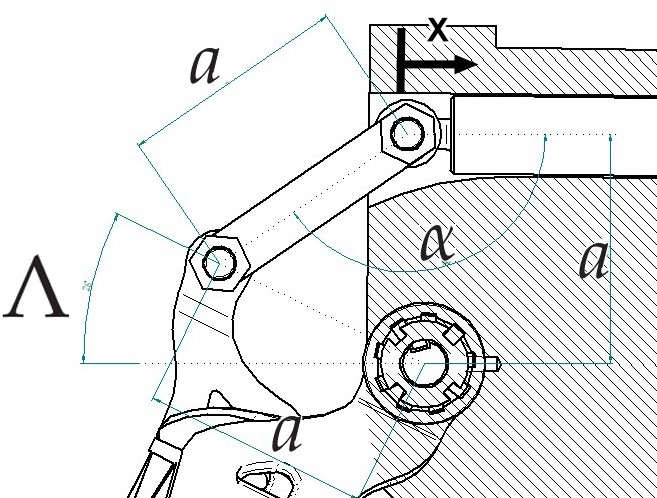
\includegraphics[width=0.6\textwidth]{KinKlapp.jpg}
	\caption{Kinematischer Zusammenhang von Hubweg und Klappwinkel}
	\label{abb_kinklapp}
\end{figure}\\
\begin{figure}[h] 
	\centering
	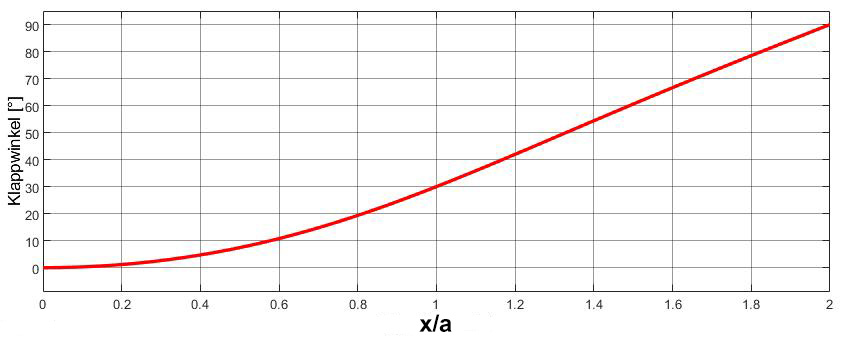
\includegraphics[width=0.9\textwidth]{KinKlappGraph.jpg}
	\caption{Klappwinkel $\Lambda$ in Abhängigkeit vom normalisierten Hubweg $x/a$}
	\label{abb_KinKlappGraph}
\end{figure}\\	
Sobald der Klappwinkel von $\Lambda = 90^\circ$ erreicht wird, beziehungsweise wenn die Hubstange sich um eine Länge von $x = 2a = 94$mm bewegt hat, stößt sie gegen das Getriebe und eine weitere Bewegung in diese Richtung ist nicht mehr möglich. Wenn dieser Fall eintritt, wird die Spannung am Motor auf null gesetzt und das Manöver gilt als beendet.
\\
Abbildung \ref{abb_KinKlappGraph} zeigt, dass der Verlauf des Klappwinkel in Abhängigkeit vom normalisieren Hubweg $x/a$ erst mit nur sehr geringer Steigung beginnt, doch dann ab $x/a \approx 0.8$ einen fast linearen Verlauf annimmt. Sowohl das Trägheitsmoment, mit dem der Grid Fin im Subsystem der Differenzialgleichung wirkt, als auch die Kraft in den Lagern, die zur Reibung führt, hängen vom aktuellen Klappwinkel ab und sind somit nicht konstant. Da jedoch schon der Klappwinkel rekursiv errechnet werden muss, ist es nicht möglich in Simulink einen weiteren geschlossenen Kreis mit diesem Wert zu bilden. Stattdessen werden Vereinfachungen angenommen. Es wird die lineare Steigung im hinteren Bereich des Verlaufs aus Abbildung \ref{abb_KinKlappGraph} als konstanter Wert für die Rechnung verwendet. Dies ist eine konservative Annahme, da die geringere Steigung im vorderen Bereich nur schwächere Reibungskräfte und Trägheitsmomente bewirken würde. Die Kraft in den beiden Kugellagern ergibt sich aus dem Trägheitsmoment des Grid Fins mit der Annahme eines Ausklappens innerhalb von zwei Sekunden und es wird angenommen, dass in beiden Lagern das gesamte Moment mit dem Hebelarm $a$ aufnehmen. Da außer der Trägheit in der Schwerelosigkeit keine Kräfte wirken, wird davon ausgegangen, dass die Reibung im Linearlager zu vernachlässigen ist. Wegen des geringen Reibungsbeiwertes $\mu = 0.0015$ \cite{lagerreibung} von Kugellagern, ist die Reibung im Getriebe mit drei Größenordnungen größeren Werten von deutlich entscheidenderer Bedeutung.
\begin{figure}[h] 
	\centering
	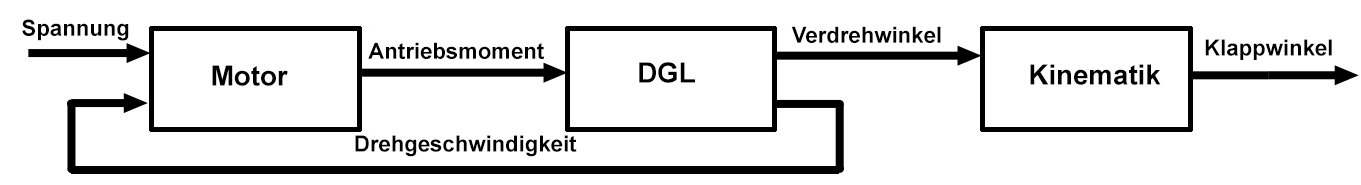
\includegraphics[width=\textwidth]{Schaubild Klapp.png}
	\caption{Schaubild der Strecke der Klappaktuatorik}
\end{figure}\\
Wird nun die Simulation mit der Nennspannung von $u = 12$V durchgeführt, klappt der Grid Fin innerhalb von weniger als 3,1 Sekunden aus. Dies liegt weit unter der Zeitspanne zwischen Separation und ReEntry-Burn, die maximal zur Verfügung steht. Der Motor ist für die Anwendung also eigentlich zu leistungsstark. Da jedoch trotz der reduzierten Masse des Grid Fins kein anderes Spindelgetriebe in Frage kommt, ist dieser Motor noch immer die günstigste Option.
\\
Als Effizienz $\mu$ des Getriebes ist jedoch nur ein Maximalwert gegeben, der hier auch verwendet wurde. Selbst wenn dieser von $\mu = 0,75$ auf einen sehr niedrigen Wert von $0,25$ herabgesetzt wird und nur noch eine Spannung von $U = 4$V am Motor anliegt, klappt der Grid Fin noch immer innerhalb von ungefähr 9 Sekunden aus.
\begin{figure}[h] 
	\centering
	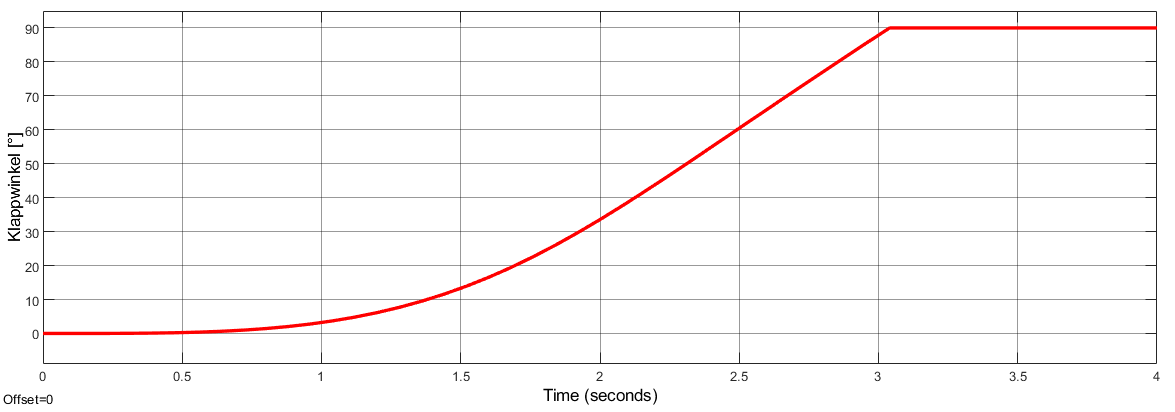
\includegraphics[width=0.8\textwidth]{Klapp1.png}
	\caption{Klappbewegung unter Normalbedingungen}
\end{figure}
\begin{figure}[h] 
	\centering
	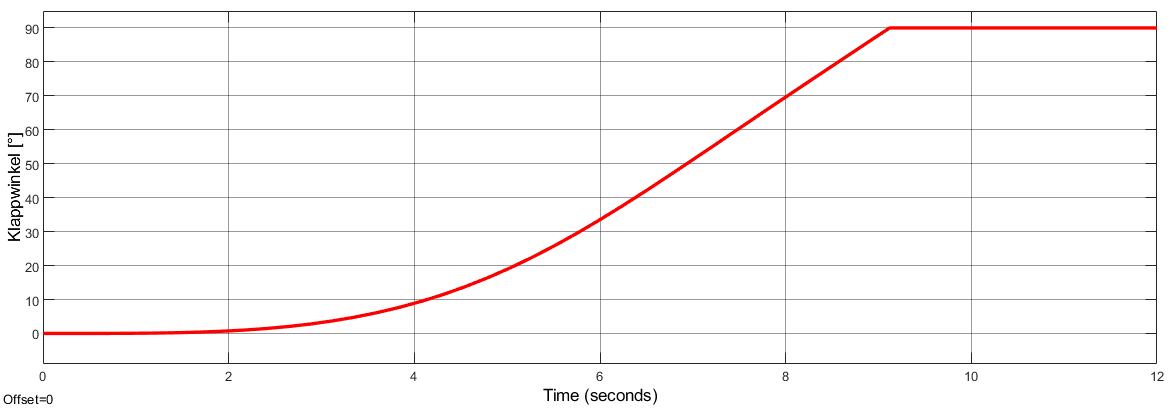
\includegraphics[width=0.8\textwidth]{Klapp2.png}
	\caption{Klappbewegung unter erschwerten Bedingungen}
\end{figure}
\subsection{Steuerwinkel}
Für den Steuerwinkel ist das erste Subsystem, der Motor, vom Aufbau her identisch und kann ohne Weiteres übernommen werden. Auch die Differenzialgleichung hat grob die gleiche Struktur.
\begin{equation}
	I\ddot{\delta} = M_{Antrieb} - M_{R} - M_{m}
\end{equation}
Zu den Momenten, die auch schon beim Klappwinkel vorkamen, kommt nun auch das aerodynamische Gelenkmoment $M_m$ dazu. Dieses wird als linear vom Steuerwinkel $\delta$ abhängig angenommen, was sich bei den Analysen von Miller und Washington \cite{synopsis} (vgl. Abbildung \ref{abb_krumm}) erkennen lässt. Somit ergibt sich
\begin{equation}
	M_{m} = \frac{M_{m, \mathrm{max}}}{\delta_\mathrm{max}} \cdot \delta =\frac{89,7\mathrm{Nm}}{20^\circ} \cdot \delta = 4,455\frac{\mathrm{Nm}}{^\circ}\cdot \delta.
\end{equation}
Der Anteil des Reibungsmoments aus der Lagerreibung lässt sich für den Steuerwinkel auch einfacher ermitteln, da sie sich aus den am Grid Fin angreifenden Kräften bestimmen lassen. Hierfür können die in Abschnitt \ref{sec:lagerWelle} zur Lagerung der Welle verwendeten Formeln \ref{eq_lagerWelle1} und \ref{eq_lagerWelle1} verwendet werden. Auch wenn der Reibungsbeiwert von Kegelrollenlagern leicht höher ist als der von Rillenkugellagern \cite{lagerreibung}, ist die Bedeutung der Lagerreibung gegenüber den Verlusten im Getriebe noch immer vernachlässigbar gering.

Da die Variable der Differenzialgleichung schon der gewünschte Steuerwinkel $\delta$ ist, ist kein drittes Subsystem für eine Transformation der Kinematik nötig. Die Bewegung, die durchgeführt werden soll, ist jedoch komplexer, als beim Klappwinkel, sodass die anliegende Spannung nicht konstant gehalten werden kann. Deswegen wird ein PI-Regler eingebaut, der in Abhängigkeit vom Steuerwinkel die Spannung regelt.
Weil eine komplette Schwingung innerhalb von $T = 0,73$s stattfinden soll, wird der Sollwert für den Steuerwinkel bis $t = 1/4T$ auf $\delta = 20^\circ$ gesetzt. Danach springt der Wert auf $\delta = -20^\circ$ und ab $t = 3/4T$ soll Steuerwinkel wieder auf $\delta = 0^\circ$ zurück gehen, wo er auch mit einer Drehrate von $\dot{\delta} = 0$ rad/s gestartet ist.
Der Regel ist jedoch keines Wegs für die Anwendung optimiert und dient nur der Demonstration der Fähigkeit des Motors genug Leistung um dieses Manöver durchzuführen aufzubringen.
\begin{figure}[h] 
	\centering
	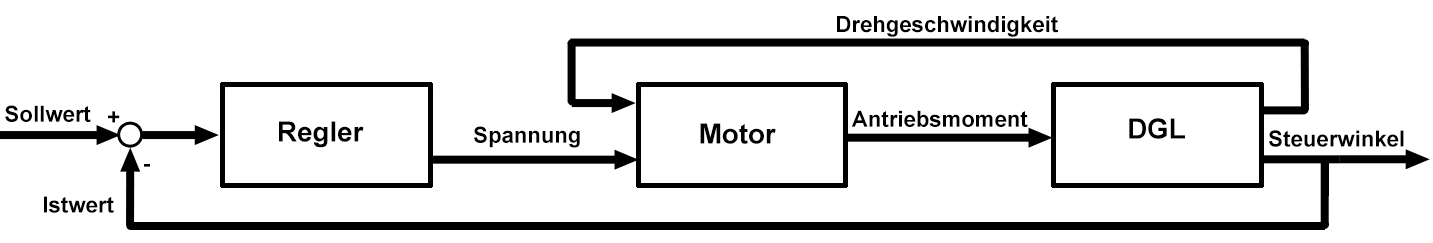
\includegraphics[width=\textwidth]{Schaubild Steuer.png}
	\caption{Schaubild der Regelstrecke der Steueraktuatorik}
\end{figure}\\
Der gewählte Motor hat eine Nennspannung von $U = 12$V, die zunächst als Maximum festgelegt wird. Unter diesen Bedingungen schafft der Motor aber gerade mal einen Steuerwinkel von $\delta = \pm 12^\circ$ einzustellen.
\begin{figure}[h] 
	\centering
	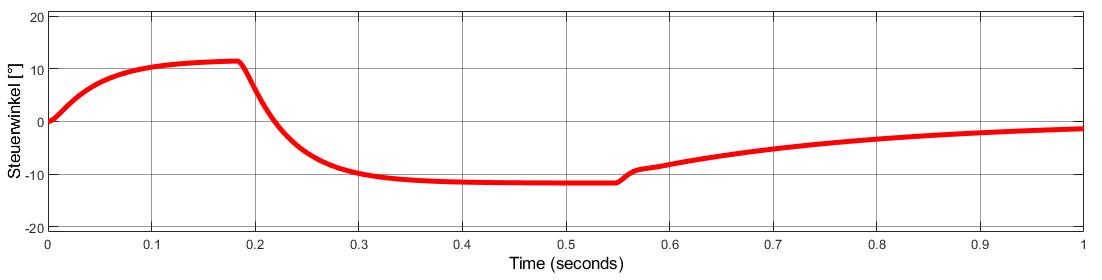
\includegraphics[width=\textwidth]{Steuer12V.png}
	\caption{Steuerwinkel in Abhängigkeit von der Zeit bei Nennspannung}
\end{figure}\\
 Jedoch ist die Nennspannung nur für den Dauerbetrieb als Grenzwert anzusehen. Da aber der Wiedereintritt in die Atmosphäre, wo dieses Manöver durchgeführt wird, nur circa 40 Sekunden dauert, wobei nur in einem Intervall von ungefähr 20 Sekunden die hohen aerodynamischen Kräfte auftreten, ist die meiste Zeit gar nicht eine so hohe Leistung notwendig. Mit einer thermischen Zeitkonstante der Wicklung von $11,8$s ist ein Überschreiten der Nennspannung um ihr Vielfaches nicht sofort schädlich. Deutlich höher muss die Spannung aber auch gar nicht gesteigert werden. Wie Abbildung \ref{abb_Steuer18V} zeigt, reicht schon eine Spannung vom 1,5-fachen der Nennspannung aus, um die Bewegung wie gewünscht durchzuführen. Er ist aber deutlich sensibler gegenüber unerwarteten Störungen als der Klappaktuator. Bei geringerer Maximalspannung und einer Senkung der Getriebeeffizienz um mehr als 5\% kann er unter den Maximalbedingungen nicht mehr die gewünschte Bewegung ausführen.
\begin{figure}[h] 
\centering
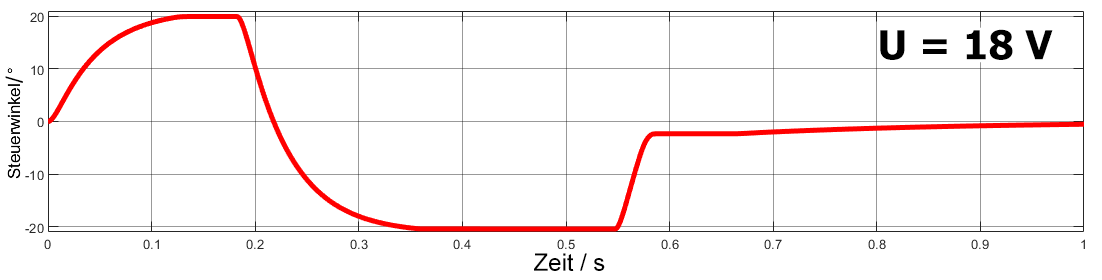
\includegraphics[width=\textwidth]{Steuer18V.png}
\caption{Steuerwinkel in Abhängigkeit von der Zeit bei 1,5-facher Nennspannung}
\label{abb_Steuer18V}
\end{figure}\\
\section{Systembewertung und Fazit}
Es wurde ein System, eine Grid Fin Aktuatorik für wiederverwendbare Raketen, die unter extremen Wiedereintrittsbedingungen einsatzfähig bleibt, entworfen. Nicht nur der Grid Fin an sich hält den mechanischen Belastungen stand, die durch die aerodynamischen Kräfte bewirkt werden, sondern auch die Bauteile, an denen er befestigt ist, können diese Spannungen ertragen und in den Raketenkörper weiterleiten. Dabei wird nicht von einem planmäßigen Wiedereintritt mit ReEntry-Burn ausgegangen, sondern das Worst-Case-Szenario angenommen, bei dem die Rakete ungebremst auf die Atmosphäre trifft. Das größte Bedenken gilt hierbei der thermischen Belastung, die weiterhin eine große Unbekannte ist. Sie konnte bisher noch nicht berücksichtigt werden und könnte somit zum Totalversagen des Systems durch Schmelzen des Gittermaterials führen.
\\~\\
Das System muss aber nicht nur den Belastungen standhalten, sondern auch eine Beweglichkeit um zwei Achsen in bestimmten Grenzen erlauben. Der erste Aktuator steuert den Grid Fin beim Wiedereintritt und schafft es selbst bei den harschen Bedingungen ohne ReEntry-Burn eine Bewegung von $\pm 20^\circ$  innerhalb von weniger als 0,73 Sekunden auszuführen. Obwohl er nur recht knapp ausgelegt ist und schon bei leicht erschwerten Bedingungen nicht mehr in der Lage ist, die Bewegung auszuführen, wird er dennoch den Anforderungen gerecht. Der Aktuator zum Ausklappen der Grid Fins nach der Stageseperation und vor dem Wiedereintritt ist deutlich robuster ausgelegt. Er schafft es innerhalb kürzester Zeit seine Funktion zu erfüllen und danach die Position zu halten. Dieser Aktuator kann auch noch bei deutlich erschwerten Bedingungen seine Aufgabe erfüllen.
\\~\\
Auch wenn einige Komponenten natürlich maßgefertigt werden müssen, insbesondere der Grid Fin, die Welle und das Gehäuse, wurden so weit wie möglich COTS verwendet. So sind die Motoren, Getriebe und Lager alle von Anbietern online bestellbar, ganz abgesehen von den Normbauteilen, die wie Schrauben und Mutter teilweise sogar aus dem lokalen Baumarkt in geringen Stückzahlen erhältlich sind. Die restlichen Bauteile sind aus einfachen Halbzeugen mit nur wenigen Arbeitsschritten fertigbar. Dadurch werden Kosten auf ein Minimum begrenzt. Für COTS ergeben sich somit pro Grid Fin Gesamtkosten von circa 1900€. Die Gesamtmasse pro Aktuatorik beläuft sich auf ungefähr $14,5$kg.
\\~\\
Zusammenfassend lässt sich sagen, dass die Aktuatorik alle geforderten Funktionen erfüllt. Sie hält allen zu berücksichtigenden Belastungen stand und ermöglicht die Bewegung der geforderten Freiheitsgrade. Somit wurden alle Forderungen aus der Aufgabenstellung als erfüllt.
